\chapter{Valutazione sperimentale delle prestazioni}
In questo capitolo analizzeremo nel dettaglio l'applicazione da me realizzata per lo svolgimento dei test su tale tecnologia.

\section{Applicazione}
Per la realizzazione dei test relativi Packet Delivery Ratio e Throughput sono stati impiegati 2 dispositivi, mentre invece per il calcolo del Discovery Time da 2 a 4 dispositivi.
Il primo dispositivo avrà la funzione di P2P Group Owner (Server), mentre invece il secondo avrà la funzione di Client.

\subsection{P2P Group Owner}
I test sono stati eseguiti con l'ausilio di un gruppo standard:
L'utilizzo di tale gruppo, come spiegato precedentemente, implica che prima che venga deciso quale dei due dispositivi sarà il Group Owner (GO), bisognerà attraversare un fase chiamata di negoziazione (GO Negotiation), in tale fase i due dispositivi decideranno su quale canale (1,6,11) porsi, ed inizieranno ad inviarsi valori numerici tra loro che dichiareranno in seguito.
Alla fine chi avrà dichiarato il valore più alto assumerà il ruolo di Grou Owner ed inizieranno a comunicare.

La comunicazione lato server avviene tramite la creazione di un Thread chiamato ThreadCalcoli (in cui verranno effettuati i calcoli delle due metriche: Packet Delivery Ratio e Throughput) che a sua volta creerà un secondo Thread chiamato ThreadComunicazione (che si occuperà esclusivamente di ricevere e reinviare i pacchetti ottenuti dal Client).
Una volta creato il ThreadComunicazione, il ThreadCalcoli andrà in stato di sleep per un totale di 50 secondi.
Tale Thread invece rimarrà in attesa dei pacchetti che verranno inviati dal Client.
Durante il processo, sono state istanziate 2 variabili che saranno fondamentali per il calcolo delle 2 metriche e che verranno condivise tra i 2 Thread.
La prima variabile sarà utile a ricavare il Throughput su 50 secondi, assumendo il valore della dimensione del pacchetto ricevuto, mentre invece la seconda avrà lo scopo di contatore per tenere traccia del numero di pacchetti ricevuti, utile per calcolare il Packet Delivery Ratio.
Una volta che il ThreadCalcoli ha raggiunto i 50 secondi, invia un segnale al ThreadComunicazione bloccandolo, permettendo così il calcolo delle 2 metriche attraverso la lettura dei dati ricevuti contenuti nelle 2 variabili.
Terminati tali calcoli il ThreadCalcoli sblocca il ThreadComunicazione e si rimette in stato di sleep per altri 50 secondi ripetendo successivamente le stesse operazioni per i cicli successivi.

\subsection{Client}
Tale dispositivo si occupa di inviare i pacchetti al Server, l'invio di tali pacchetti avviene attraverso la lettura di un array chiamato packets che contiene il numero di pacchetti da inviare.


\section{Dispositivi usati}
Per la realizzazione di tali esperimenti sono stati usati i seguenti dispositivi:

-Samsung Galaxy S5

\begin{center}
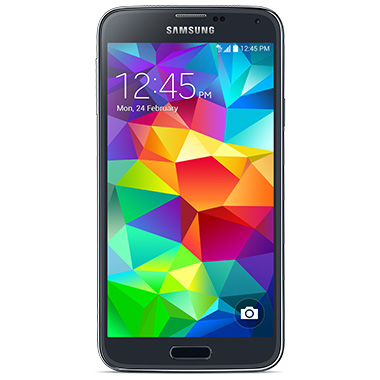
\includegraphics[width=1\textwidth]{imgs/s5.jpg}
\captionof{figure}{Samsung Galaxy S5}\label{s5_img}%
\end{center}
\newpage

-Google Nexus 5

\begin{center}
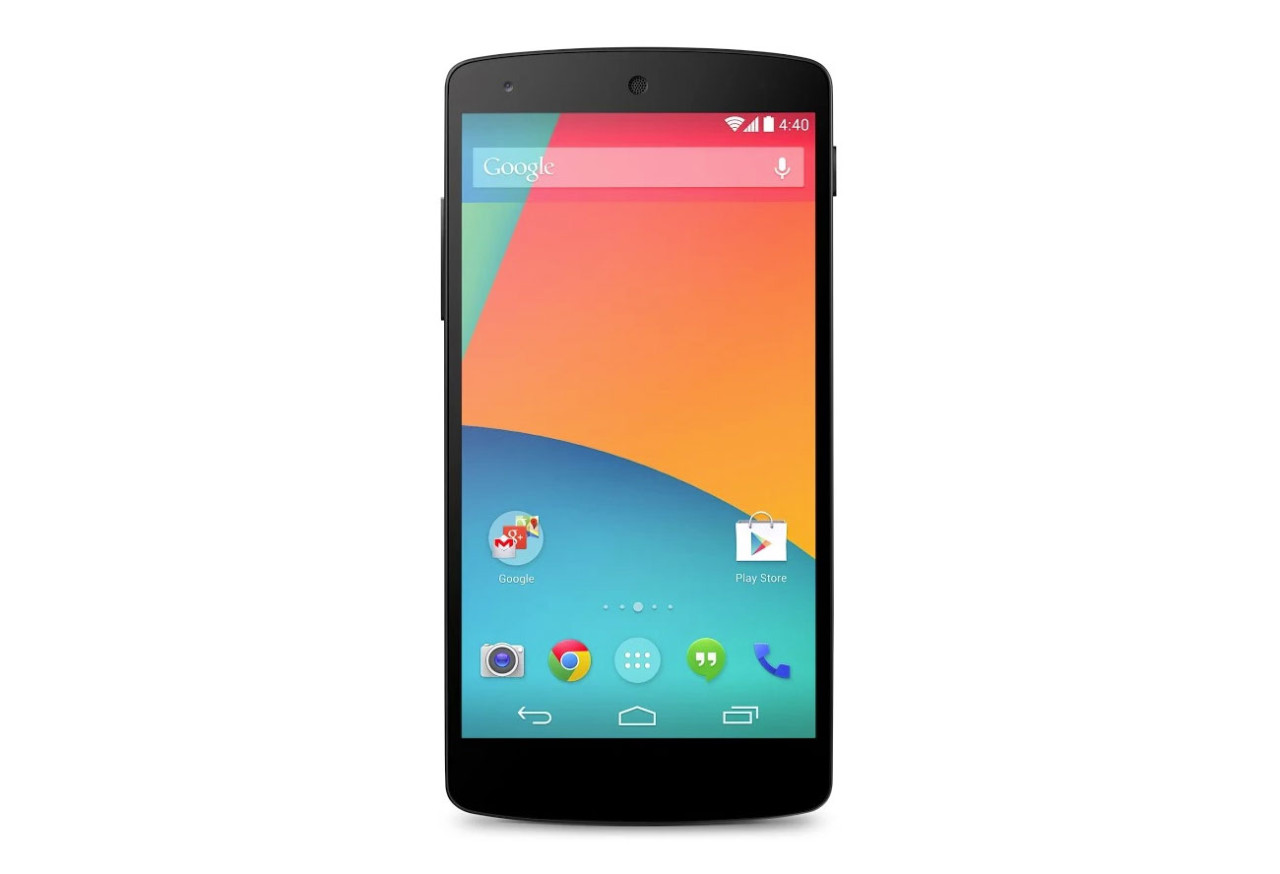
\includegraphics[width=1\textwidth]{imgs/nexus5.jpg}
\captionof{figure}{Google Nexus 5}\label{nexus_5_img}%
\end{center}
\newpage

-Samsung Galaxy S3

\begin{center}
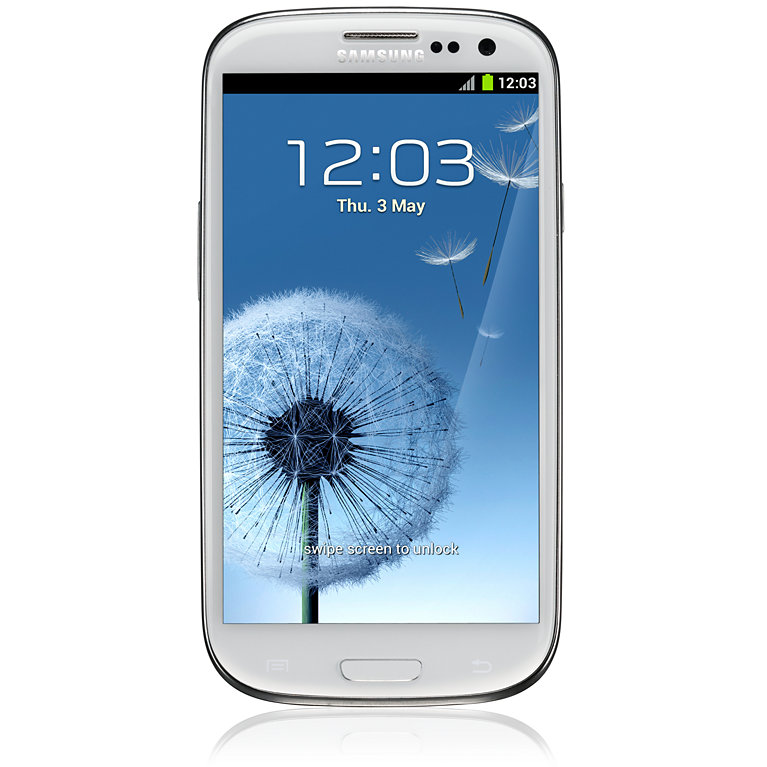
\includegraphics[width=1\textwidth]{imgs/galaxy_s3.jpg}
\captionof{figure}{Samsung Galaxy S3}\label{galaxys3_img}%
\end{center}
\newpage

-Samsung Galaxy Tab 2

\begin{center}
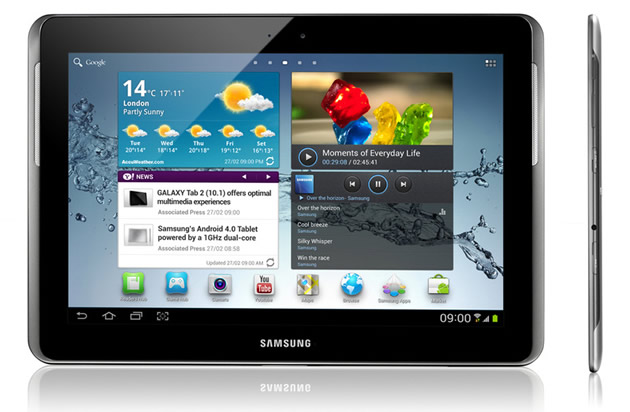
\includegraphics[width=1\textwidth]{imgs/galaxy_tab_2.jpg}
\captionof{figure}{Samsung Galaxy Tab 2}\label{galaxy_tab_2_img}%
\end{center}

\section{Esperimenti}
Per effettuare il calcolo delle 3 metriche ho eseguito i test in 2 ambienti:Indoor e Outdoor.

\subsection{Packet Delivery Ratio (PDR) e Throughput}

Per eseguire il calcolo del Packet Delivery Ratio ho impostato un array packets con una serie di valori che indicano il numero di pacchetti da inviare.

Per quanto riguarda invece il calcolo del Throughput ho impostato un tempo pari a 50 secondi e una dimensione del singolo pacchetto di 1000 Byte.
Il test quindi ha 9 cicli della durata di 50 secondi con un numero di pacchetti diverso ad ogni ciclo.
Per tutti e due i test la distanza tra i due dispositivi viene variata continuamente.
Nele immagini di seguito viene illustrato il procedimento:

\begin{center}
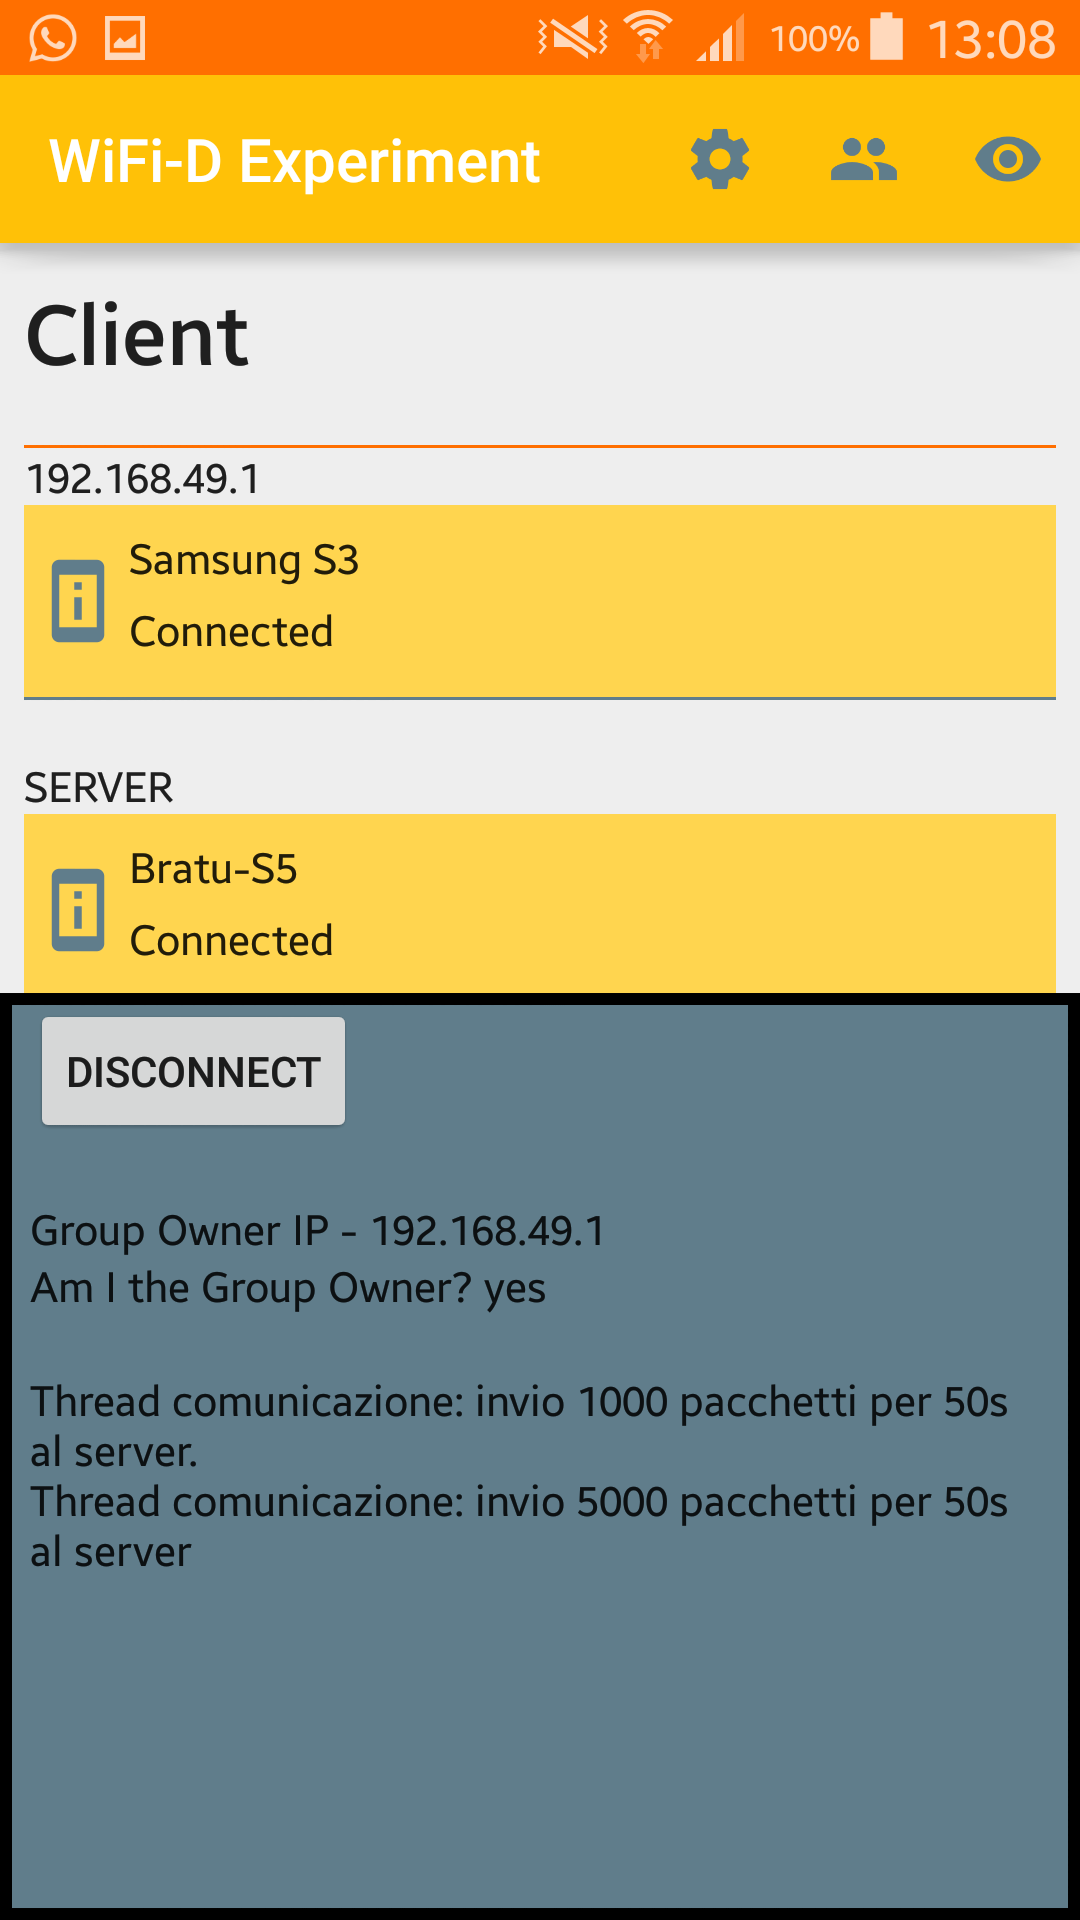
\includegraphics[width=0.5\textwidth]{imgs/Client.png}
\captionof{figure}{Il client invia i pacchetti al Server}\label{client_img}%
\end{center}

\begin{center}
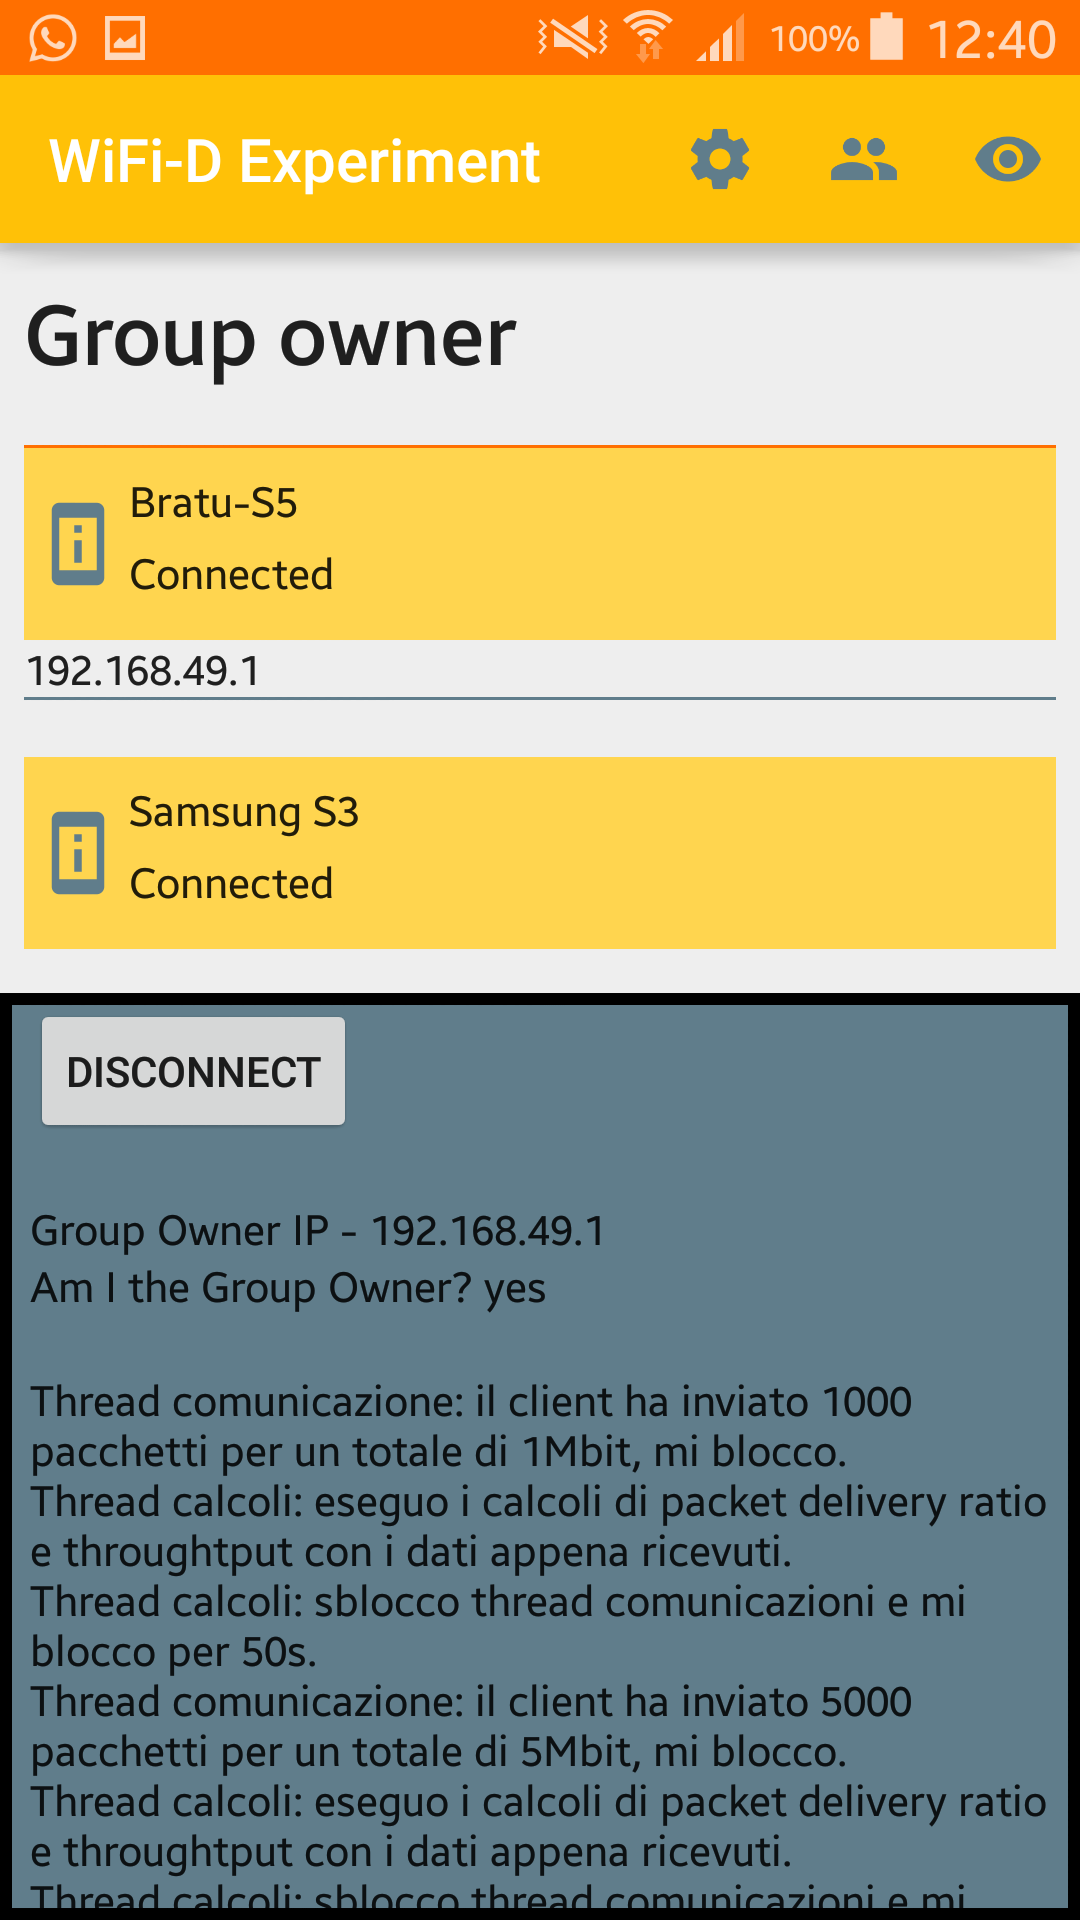
\includegraphics[width=0.5\textwidth]{imgs/Server.png}
\captionof{figure}{Il server riceve e re-invia i pacchetti al Client, occupandosi in parallelo di fare il calcolo delle metriche}\label{server_img}%
\end{center}



\subsection{Discovery Time}

Per eseguire il calcolo di tale metrica ho usufruito di 2 tipologie di gruppi per la decisione del Group Owner: Gruppo standard e Gruppo Autonomo.
Nel caso del gruppo standard l'associazione tra i due dispositivi avviene tramite una semplice discovery (attivabile tramite l'apposito pulsante a forma di occhio in alto a destra, che implicherà però il passaggio attraverso una fase di GO Negotiation per decidere chi sarà Group Owner.


\begin{center}
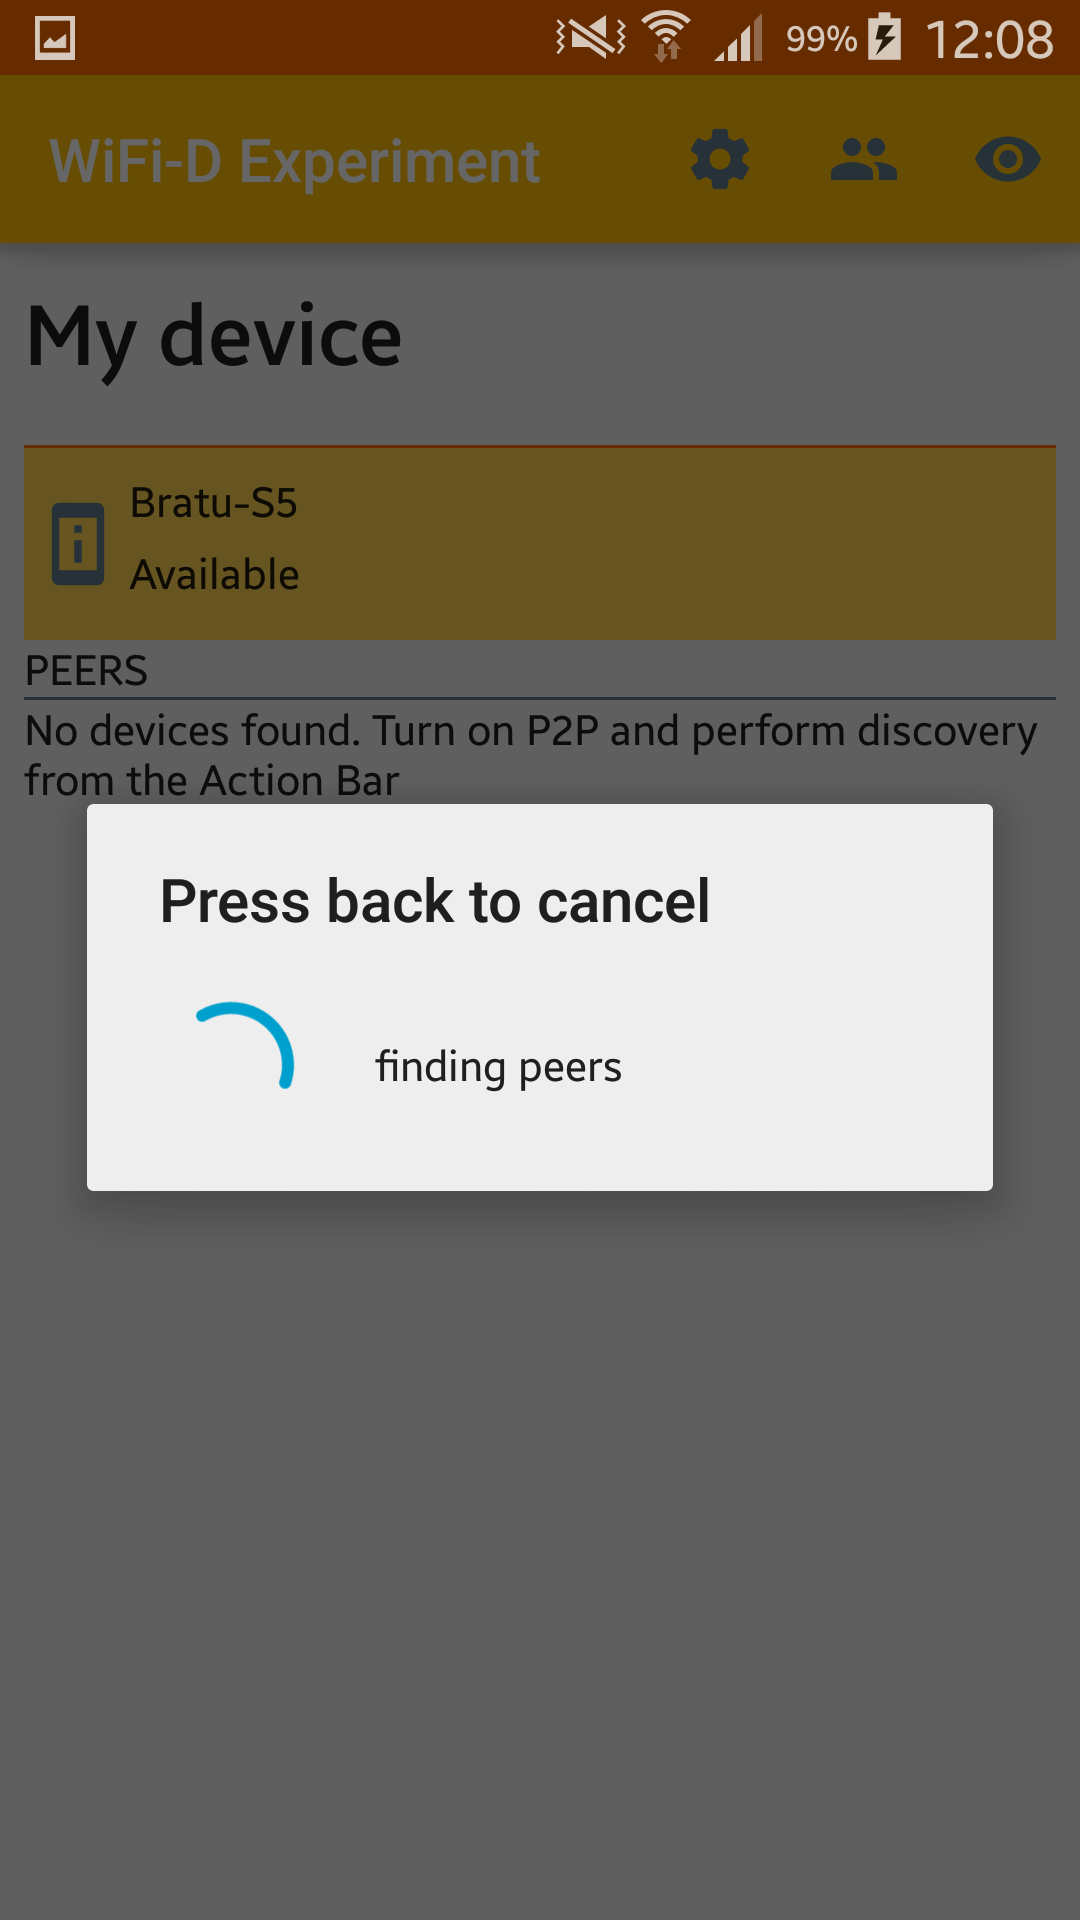
\includegraphics[width=0.5\textwidth]{imgs/Discovery.png}
\captionof{figure}{Cliccando sul pulsante a forma di occhio partirà la discovery}\label{discovery_img}%
\end{center}

Una volta trovato il dispositivi a cui connettersi, comparirà una finestra col tempo impiegato, figura \ref{tempo_discovery_img}.

\begin{center}
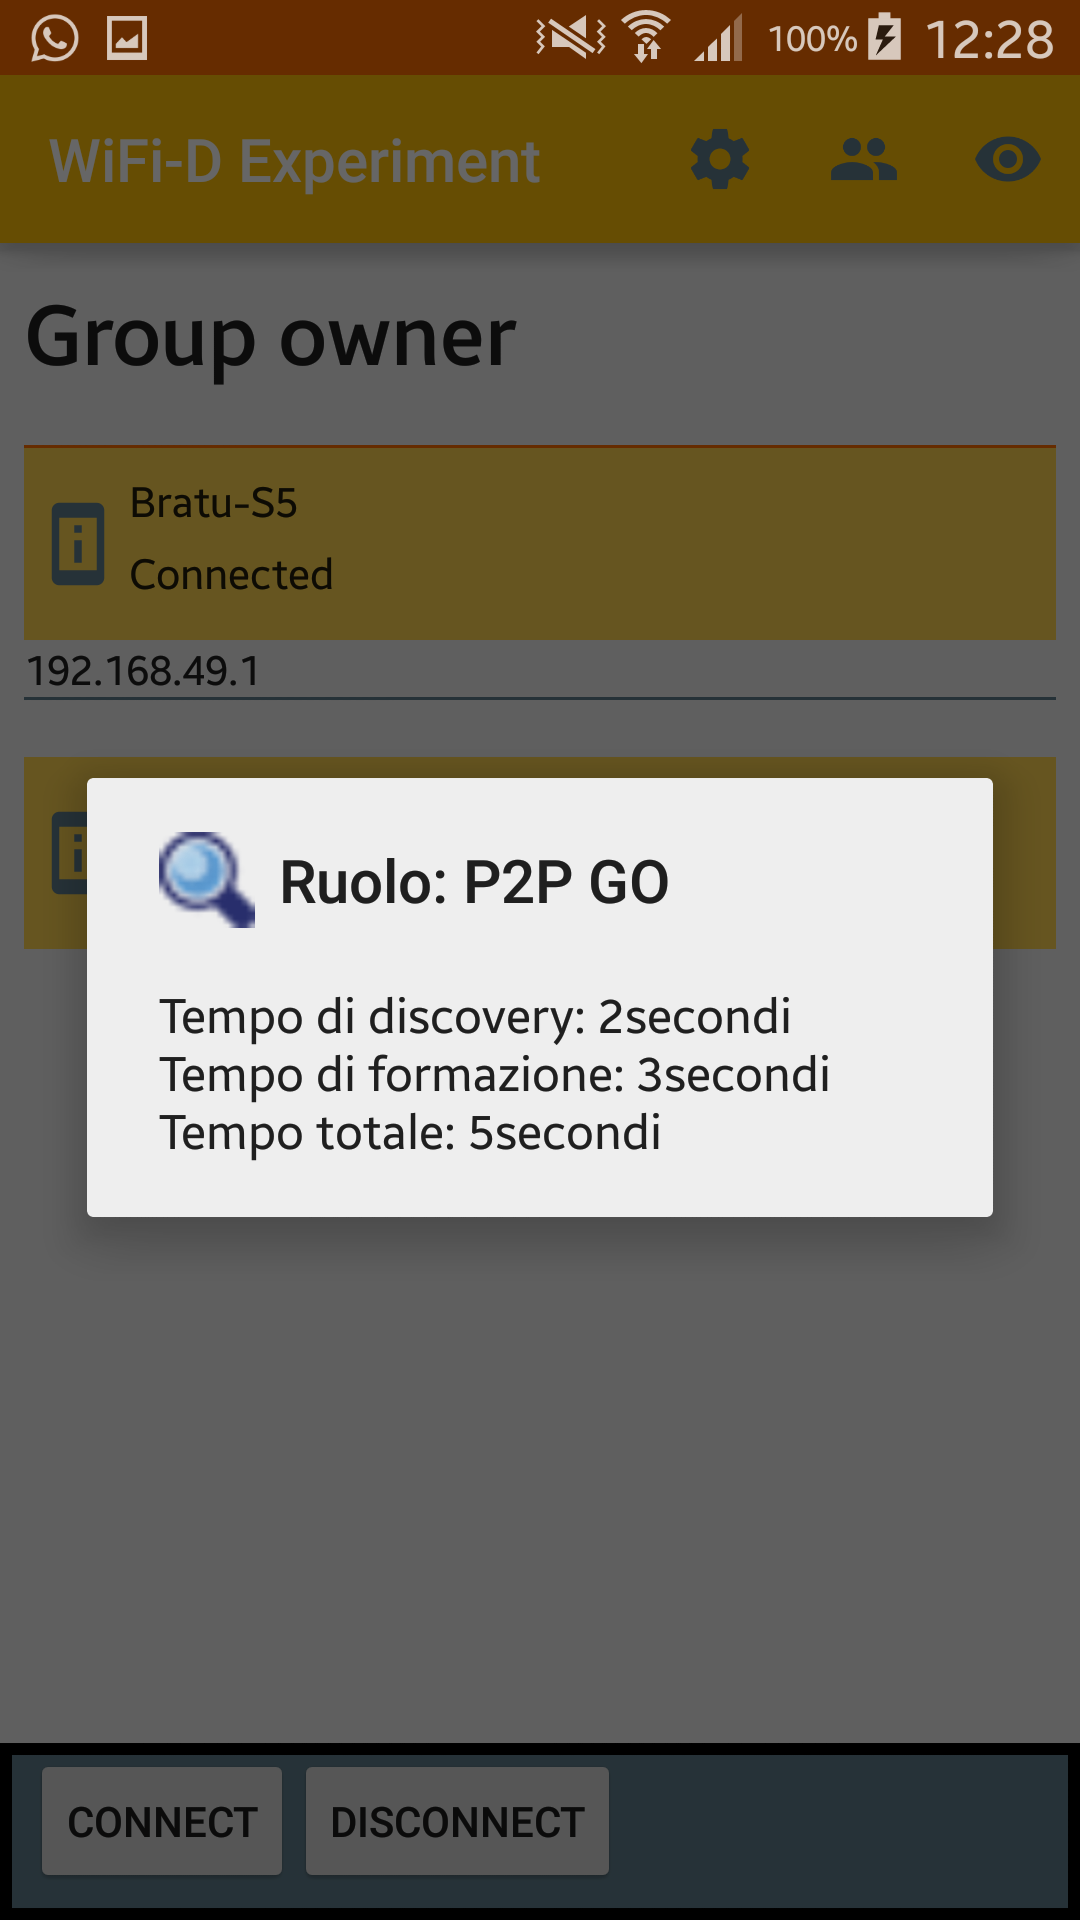
\includegraphics[width=0.5\textwidth]{imgs/tempo_discovery.png}
\captionof{figure}{Il tempo impiegato per la ricerca e l'associazione}\label{tempo_discovery_img}%
\end{center}


Nel caso del gruppo autonomo invece, tale fase non viene eseguita, e quindi il dispositivo diventerà subito il Group Owner e gli altri potranno associarsi tramite una semplice discovery, per usufruire del gruppo autonomo basterà cliccare sul pulsante apposito raffigurante 2 persone e il dispositivo assumerà subito il ruolo di Group Owner.
Nel calcolo di tale metrica è stato effettuato anche un ulteriore esperimento connettendo tra loro più dispositivi figura \ref{piu_dispositivi_img}.

\begin{center}
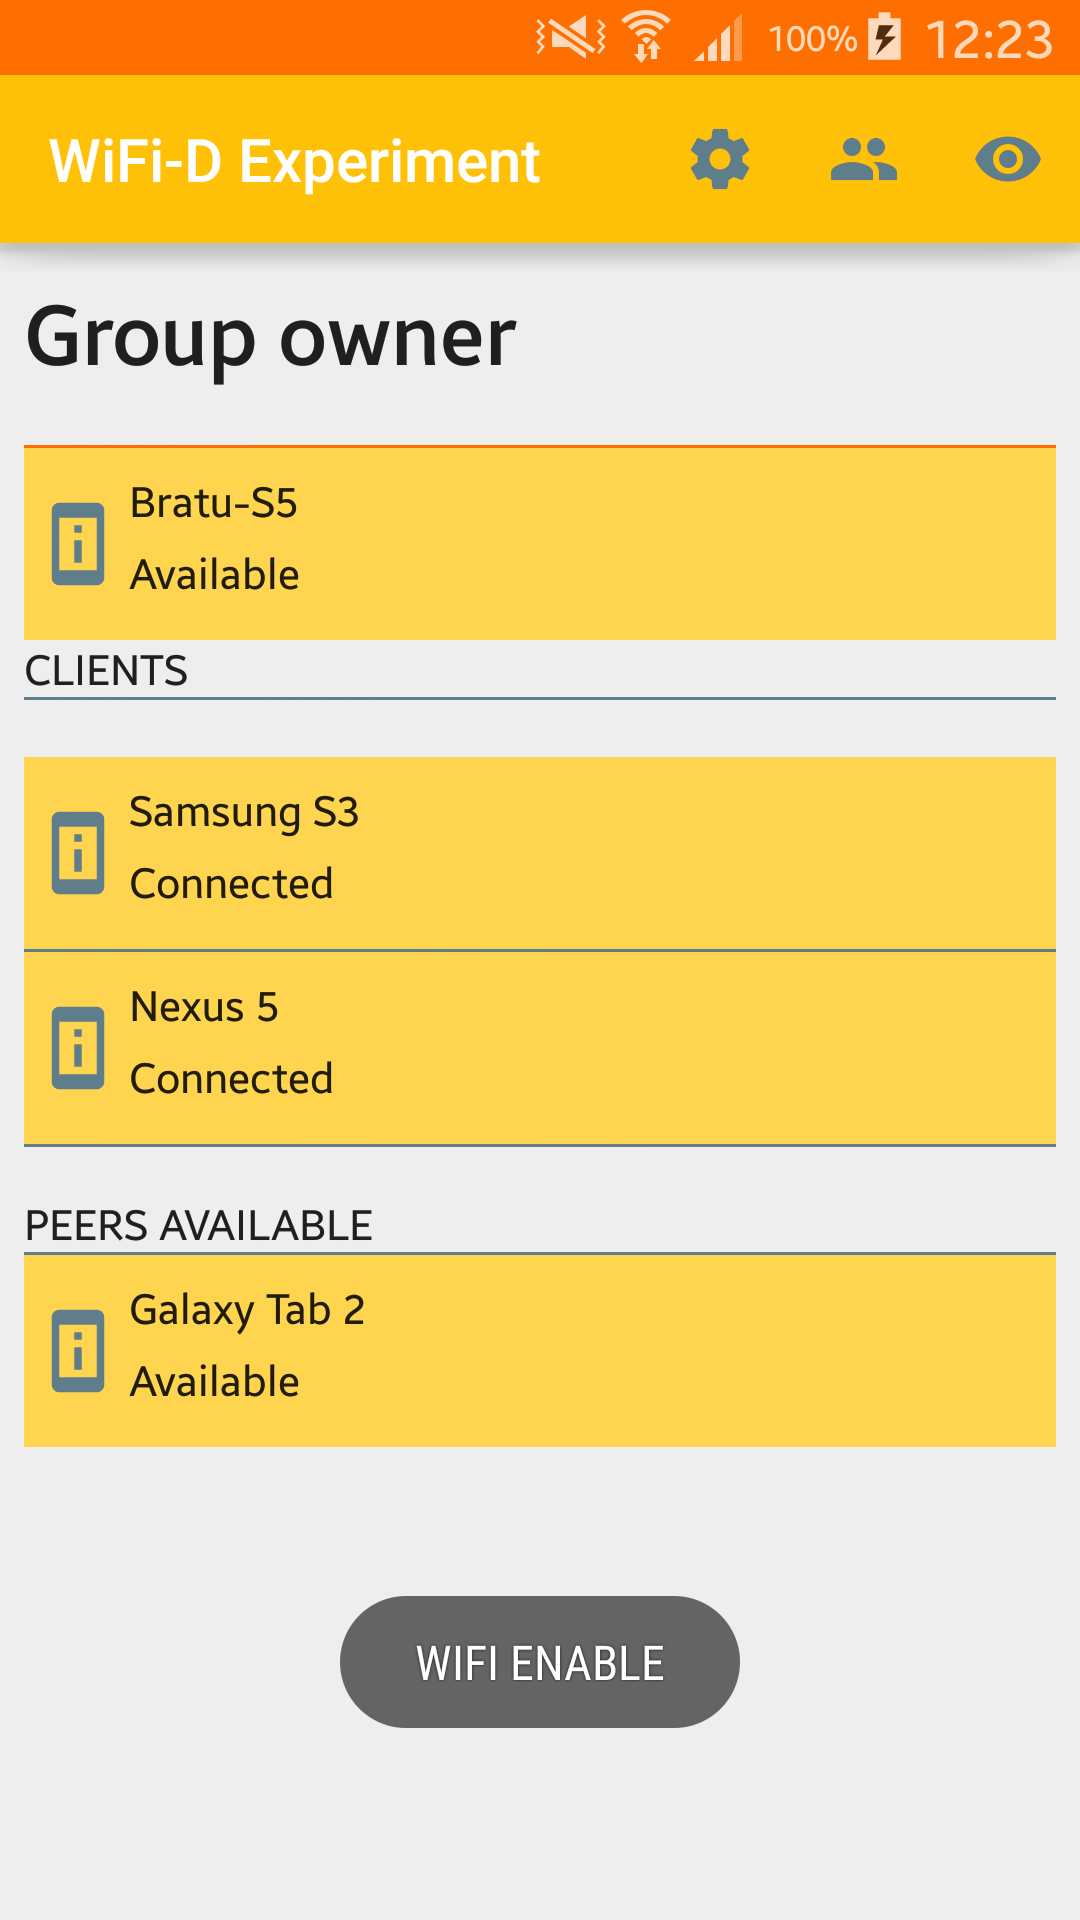
\includegraphics[width=0.5\textwidth]{imgs/piu_dispositivi.png}
\captionof{figure}{Il tempo impiegato per la ricerca e l'associazione tra i dispositivi}\label{piu_dispositivi_img}%
\end{center}
\newpage


\section{Metriche}
Qui di seguito riporterò le formule utilizzate per il calcolo delle 3 metriche.

\subsection{Packet Delivery Ratio (PDR)}
\begin{center}
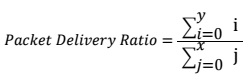
\includegraphics[width=1\textwidth]{imgs/PDR.jpg}
\captionof{figure}{Formula calcolo Packet Delivery Ratio}\label{PDR_img}%
\end{center}

Rapporto fra il numero di pacchetti ricevuti a destinazione e il numero di pacchetti inviati dalla sorgente.
Dove x rappresenta il numero di pacchetti inviati dalla sorgente e y il numero di quelli ricevuti a destinazione figura \ref{PDR_img}. 

\subsection{Throughput}
\begin{center}
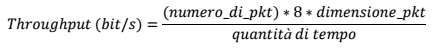
\includegraphics[width=1\textwidth]{imgs/Throughput.jpg}
\captionof{figure}{Formula calcolo Throughput}\label{Throughput_img}%
\end{center}

Rappresenta l’effettiva quantità di byte trasmessi in una determinata quantità di tempo figura \ref{Throughput_img}.
Negli esperimenti è stato considerato un tempo di 50 secondi e una dimensione dei pacchetti di 1000 Byte.

\subsection{Discovery Time}

Il calcolo del Discovery Time indica il tempo impiegato dai 2 dispositivi per trovarsi e associarsi.

Tale calcolo è stato fatto eseguendo la fase di Discovery per 30 volte per ogni singola distanza, successivamente si è eseguito un semplice calcolo della media prendendo e sommando tutti i valori uguali ( esempio se per più volte abbiamo ottenuto un tempo di 5 secondi sarà: 5+5+5+5.... ) e dividendoli per 30, tale risultato verrà poi trasformato in percentuale.




\clearpage{\pagestyle{empty}\cleardoublepage}